\documentclass[10pt,openany]{book}\usepackage[]{graphicx}\usepackage[]{color}
% maxwidth is the original width if it is less than linewidth
% otherwise use linewidth (to make sure the graphics do not exceed the margin)
\makeatletter
\def\maxwidth{ %
  \ifdim\Gin@nat@width>\linewidth
    \linewidth
  \else
    \Gin@nat@width
  \fi
}
\makeatother

\definecolor{fgcolor}{rgb}{0.345, 0.345, 0.345}
\newcommand{\hlnum}[1]{\textcolor[rgb]{0.686,0.059,0.569}{#1}}%
\newcommand{\hlstr}[1]{\textcolor[rgb]{0.192,0.494,0.8}{#1}}%
\newcommand{\hlcom}[1]{\textcolor[rgb]{0.678,0.584,0.686}{\textit{#1}}}%
\newcommand{\hlopt}[1]{\textcolor[rgb]{0,0,0}{#1}}%
\newcommand{\hlstd}[1]{\textcolor[rgb]{0.345,0.345,0.345}{#1}}%
\newcommand{\hlkwa}[1]{\textcolor[rgb]{0.161,0.373,0.58}{\textbf{#1}}}%
\newcommand{\hlkwb}[1]{\textcolor[rgb]{0.69,0.353,0.396}{#1}}%
\newcommand{\hlkwc}[1]{\textcolor[rgb]{0.333,0.667,0.333}{#1}}%
\newcommand{\hlkwd}[1]{\textcolor[rgb]{0.737,0.353,0.396}{\textbf{#1}}}%
\let\hlipl\hlkwb

\usepackage{framed}
\makeatletter
\newenvironment{kframe}{%
 \def\at@end@of@kframe{}%
 \ifinner\ifhmode%
  \def\at@end@of@kframe{\end{minipage}}%
  \begin{minipage}{\columnwidth}%
 \fi\fi%
 \def\FrameCommand##1{\hskip\@totalleftmargin \hskip-\fboxsep
 \colorbox{shadecolor}{##1}\hskip-\fboxsep
     % There is no \\@totalrightmargin, so:
     \hskip-\linewidth \hskip-\@totalleftmargin \hskip\columnwidth}%
 \MakeFramed {\advance\hsize-\width
   \@totalleftmargin\z@ \linewidth\hsize
   \@setminipage}}%
 {\par\unskip\endMakeFramed%
 \at@end@of@kframe}
\makeatother

\definecolor{shadecolor}{rgb}{.97, .97, .97}
\definecolor{messagecolor}{rgb}{0, 0, 0}
\definecolor{warningcolor}{rgb}{1, 0, 1}
\definecolor{errorcolor}{rgb}{1, 0, 0}
\newenvironment{knitrout}{}{} % an empty environment to be redefined in TeX

\usepackage{alltt}

%\input{c:/aaaWork/zGnrlLatex/BookPreamble_HC}   % use for the hard-copy version
\input{c:/aaaWork/zGnrlLatex/BookPreamble}
\hypersetup{pdftitle = MTH107 Notes,bookmarksdepth=0}
\input{c:/aaaWork/zGnrlLatex/JustRPreamble}
\usepackage{animate}
\usepackage{titlesec}
\titlespacing\section{0pt}{12pt plus 4pt minus 2pt}{0pt plus 2pt minus 2pt}
\titlespacing\subsection{-3pt}{12pt plus 4pt minus 2pt}{0pt plus 2pt minus 2pt}
\titlespacing\subsubsection{-3pt}{12pt plus 4pt minus 2pt}{0pt plus 2pt minus 2pt}
\renewcommand{\chaptername}{Module}
\IfFileExists{upquote.sty}{\usepackage{upquote}}{}
\begin{document}




  \frontmatter
    %MAKE MINI TABLE OF CONTENTS for each chapter ----------------------------------
\dominitoc
\setcounter{minitocdepth}{1} %sets the depth to show in chapter TOC -- 0 is chapters, 1 would be sections, etc.

\VerbatimFootnotes  % allows verbatim in footnotes

%TITLE PAGE --------------------------------------------------------------------
\begin{titlepage}
\begin{center}

% Upper part of the page
\textsc{\LARGE Northland College}\\[0.5cm]
\textsc{\Large MTH107 -- Statistical Analysis and Interpretation}\\[1.5cm]

\HRuleW \\
\HRule \\[1cm]
{ \huge \bfseries Introduction to Statistical Analysis and Interpretation}\\[1cm]
\HRule \\
\HRuleW \\[1.5cm]

% Author and supervisor
\begin{minipage}{0.4\textwidth}
\begin{flushleft}
%  \Large \emph{Author:}\\ Dr. Derek H. Ogle
  \Large \emph{Instructors:}\\Dr. Derek H. Ogle \\ Jodi Supanich
\end{flushleft}
\end{minipage}
\begin{minipage}{0.4\textwidth}
\begin{flushright}
  \Large \emph{Department:} \\ Mathematical Sciences
%  \Large \emph{Department:} \\ Mathematical Sciences \\ Mathematical Sciences
\end{flushright}
\end{minipage}

\vfill

% Bottom of the page
%\includegraphics[width=4in]{Title.JPG} \\[2.5cm]
{\Large \today}

\end{center}

\end{titlepage}

% The material in the Preface_OLD.tex file was between here
% and here

%TABLE OF CONTENTS ---------------------------------------------------------------------------------------------------
\setcounter{tocdepth}{0} %sets the depth to show in TOC -- 0 is chapters, 1 would be sections, etc.

%modify what the parts look like
\renewcommand{\cftpartfont}{\scshape}                          %changes to small caps

%modify what the chapters look like
\setlength{\cftchapindent}{1.5em}                              %indent the chapters
\setlength{\cftbeforechapskip}{0.4em}                          %set the space between chapters -- reduce to 0.2 if depth is set to 0

%modify what the sections look like
\setlength{\cftsecindent}{3.8em}                               %indent the sections --- doesn't seem to work
\setlength{\cftbeforesecskip}{0.2em}                           %set the space between sections

\newpage                                                       %need this so that the TOC will start on its own page
\tableofcontents                                               %build the table of contents

%SETTING FOR LEAVING FRONT MATTER AND GOING TO MAIN DOCUMENT ---------------------------------------------------------
\addtocontents{toc}{\setlength{\cftbeforepartskip}{1.5em}}     %increase distance before parts in the main TOC
\addtocontents{toc}{\cftpagenumbersoff{part}}                  %so page numbers won't appear for parts in the main TOC


  \mainmatter



















\chapter{2-Sample t-Test} \label{chap:tTest2}

\vspace*{-12pt}
\minitoc
\vspace*{24pt}

\lettrine{W}{hile it is often useful to test whether a population mean} differs from a specific value (i.e., with the 1-Sample t-Test of \modref{chap:tTest1}), there are many instances where interest is in whether means from two groups (or populations) differ. For example, is there a difference in mean income between males and females, in mean test scores between students from high- and low-income families, in mean percent body fat between raccoons from southern and northern Wisconsin, or in mean amount of milk produced from cows provided with a hormone or a placebo. In all of these situations, interest is identifying if a difference in population means exists between two groups (males and females, students from high- and low-income families, raccoons from southern and northern Wisconsin, cows given a hormone or a placebo). A \textbf{2-Sample t-Test} is used in these situations and is the subject of this module.


\section{2-Sample t-Test Specifics}
\vspace*{-3pt}
In a 2-Sample t-Test, $H_{0}:\mu_{1}=\mu_{2}$ states that the two population means are equal. This can be rewritten as $H_{0}:\mu_{1}-\mu_{2}=0$, because the difference between two population means should be zero if the two population means are equal. With this $H_{0}$, the ``parameter'' is $\mu_{1}-\mu_{2}$ and the corresponding statistic is $\bar{x}_{1}-\bar{x}_{2}$. Thus, a 2-Sample t-Test is focused on the difference in population means.

When looking at the ``general'' test statistic formula (i.e., Equation \eqref{eqn:zTestStatGeneral}) of

\vspace*{-6pt}
\[ \text{Test Statistic} = \frac{\text{Observed Statistic}-\text{Hypothesized Parameter}}{SE_{\text{Statistic}}} \]
\vspace*{-6pt}

it is apparent that the SE of $\bar{x}_{1}-\bar{x}_{2}$ (i.e., the statistic) is needed. Unfortunately, the calculation of this standard error depends on whether the two population variances are equal or not. When the variances are approximately equal (discussed in \sectref{sect:LevenesTest}), the standard error of $\bar{x}_{1}-\bar{x}_{2}$ is

\[ SE_{\bar{x}_{1}-\bar{x}_{2}}= \sqrt{s_{p}^{2}\left(\frac{1}{n_{1}}+\frac{1}{n_{2}} \right)}  \]

where $n_{1}$ and $n_{2}$ are the sample sizes for the two groups and $s_{p}^{2}$ is the ``pooled sample variance'' computed as a weighted average of the two sample variances ($s_{1}^{2}$ and $s_{2}^{2}$), or

\[s_{p}^{2}=\frac{(n_{1}-1)s_{1}^{2}+(n_{2}-1)s_{2}^{2}}{n_{1}+n_{2}-2} \]

The degrees-of-freedom for the 2-Sample t-Test with equal variances come from the denominator of the pooled variance calculation; i.e., $df=n_{1}+n_{2}-2$. The specifics of the 2-Sample t-Test are in \tabref{tab:2tspec}.

\vspace*{12pt}
\begin{table}[h]
\centering
\colorbox{ltgray}{
\begin{minipage}{.8\textwidth}
  \centering
	\caption{Characteristics of a 2-Sample t-Test with equal variances.}\label{tab:2tspec}
  \begin{Itemize}
      \item \textbf{Hypothesis:} $H_{0}:\mu_{1}-\mu_{2}=0$
      \item \textbf{Statistic:} $\bar{x}_{1}-\bar{x}_{2}$
      \item \textbf{Test Statistic:} $t=\frac{\bar{x}_{1}-\bar{x}_{2}-0}{\sqrt{s_{p}^{2}\left(\frac{1}{n_{1}}+\frac{1}{n_{2}} \right)}}$ where $s_{p}^{2}=\frac{(n_{1}-1)s_{1}^{2}+(n_{2}-1)s_{2}^{2}}{n_{1}+n_{2}-2}$.
      \vspace{6pt}
      \item \textbf{Confidence Region:} $(\bar{x}_{1}-\bar{x}_{2})+t^{*}\sqrt{s_{p}^{2}\left(\frac{1}{n_{1}}+\frac{1}{n_{2}} \right)}$
      \vspace{6pt}
      \item \textbf{df:} $n_{1}+n_{2}-2$
      \item \textbf{Assumptions:} $n_{1}+n_{2}\geq40$, $n_{1}+n_{2}-2\geq15$ and \textbf{each sample} (i.e., histogram) is not strongly skewed, OR \textbf{each sample} is normally distributed.
      \item \textbf{Use with:} Quantitative response, two groups (or populations), individuals are independent between groups.
  \end{Itemize}
\end{minipage}}
\end{table}
\vspace*{12pt}

\warn{The $s_{p}^{2}$ calculation can be ``checked'' by determining if the value of $s_{p}^{2}$ is between $s_{1}^{2}$ and $s_{2}^{2}$ or if the value of $\sqrt{s_{p}^{2}}$ is between $s_{1}$ and $s_{2}$.}

A 2-Sample t-Test is often used to test an alternative hypothesis of simply finding a difference between the two groups. However, if the null hypothesis is rejected in these instances (thus, identifying a significant difference between the two groups), then care should be taken to specifically describe how the two groups differ. If the statistic is negative, then the mean of the first group is lower than the mean of the second group and, if the statistic is positive, then the mean of the first group is larger than the mean of the second group. The values of the confidence region should be used to identify how much larger or smaller the mean from one group is compared to the mean of the other group.


\newpage
\section{Testing for Equal Variances}\label{sect:LevenesTest}
As noted above, the methods of a 2-Sample t-Test differ depending on whether the two population variances are equal or not. This should present a problem to you because the population variances are parameters and are typically not known.\footnote{Actually, the population variances don't have to be known, it just needs to be known whether they are equal or not.} The question of whether these parameters are equal or not is answered with a hypothesis test, as has been done with all other questions about parameters.

A Levene's Test is used to determine whether two population variances are equal. The specifics of the Levene's test are not examined in detail here, rather you only need to know that $H_{0}:\sigma_{1}^{2}=\sigma_{2}^{2}$ is tested against $H_{A}:\sigma_{1}^{2}\neq\sigma_{2}^{2}$. We will use computer software to compute the p-value for this test (without further detail). If the Levene's Test p-value $< \alpha$, then $H_{0}$ is rejected and the population variances are considered unequal. If the p-value $> \alpha$, then $H_{0}$ is not rejected and the population variances are considered equal.


\subsection{Example - Corn and Fertilizers}
Below are the 11-steps \sectrefp{sec:11Steps} for completing a full hypothesis test for the following situation:
\vspace{-4pt}
\begin{quote}
\textsl{An agricultural researcher thought that corn plants grown in pots exposed to a certain type of synthetic fertilizer would grow taller than plants exposed to an organic fertilizer. To collect data to test this idea, he grew 50 corn plants in individual pots -- 25 were treated with organic fertilizer and 25 were treated with synthetic fertilizer. Each pot contained soil from a well-mixed common source and was planted in the same greenhouse. Each plant was similar in all regards (similar genetics, age, etc.). Use the results (heights of individual plants) in \tabref{tab:CornFert} to test the researcher's hypothesis at the 5\% level.}
\end{quote}

\vspace*{-4pt}
\begin{table}[htbp]
  \caption{Summary statistics of the corn plant height in two treatments.}
  \label{tab:CornFert}
\vspace*{-5pt}
  \begin{center}
    \begin{minipage}{4.5in}
      \begin{Verbatim}
        Synthetic  Organic
means:    51.46     47.49
SD:       5.975     6.721          Levene's Test:  p=0.1341
      \end{Verbatim}
    \end{minipage}
  \end{center}
\end{table}
\vspace*{-18pt}

\begin{Enumerate}
  \item $\alpha$ = 0.05.
  \item $H_{0}:\mu_{s}-\mu_{o} = 0$ vs $H_{A}:\mu_{s}-\mu_{o} > 0$, where $\mu$ is the mean plant height, $s$ represents synthetic fertilizer, and $o$ represents organic fertilizer. [\textit{Note that positive differences represent larger values for synthetic fertilizer; thus, $H_{A}$ represents synthetic fertilizer producing taller plants.}]
  \item A 2-Sample t-Test is required because (i) a quantitative variable (height) was measured, (ii) two groups are being compared (synthetic and organic fertilizers), and (iii) plants in the two groups were \textbf{IN}dependent as the plants were not paired, plants were not tested over time, etc.
  \item The data appear to be part of an experiment (the researcher imposed the treatments on the plants) with no clear indication of random selection of plants or random allocation of plants to the two treatments.
  \item (i) $n_{s}+n_{o}$ = 50 $> 40$, (ii) individuals in the two groups are independent as discussed above, and (iii) the population variances appear to be equal because the Levene's Test p-value (0.1341) is $> \alpha$.
  \item $\bar{x}_{s}-\bar{x}_{0}$ = 51.46 $-$ 47.49 = 3.97. Additionally,
    \[s_{p}^{2}=\frac{(25-1)5.975^{2}+(25-1)6.721^{2}}{25+25-2} = 40.44 \]
and
    \[ SE_{\bar{x}_{s}-\bar{x}_{o}}=\sqrt{40.44\left(\frac{1}{25}+\frac{1}{25} \right)} = 1.799  \]
  \item $t$ = $\frac{3.97-0}{1.799}$ = $\frac{3.97}{1.799}$ = 2.207 with 25+25-2 = 48 df.
  \item p-value = $0.0161$.
  \item The $H_{0}$ is rejected because the p-value $< \alpha$.
  \item The average height of the corn plants appears to be greater for plants grown with synthetic fertilizer than for plants grown with organic fertilizer.
  \item I am 95\% confident that plants grown with synthetic fertilizer are more than 0.95 cm taller, on average, than plants grown with the organic fertilizer. [Note $3.97-1.677*1.799$ = 3.97 $-$ 3.02 = 0.95.]
\end{Enumerate}

\begin{minipage}{\textwidth}
\textbf{R Appendix:}
\vspace{-6pt}
\begin{knitrout}
\definecolor{shadecolor}{rgb}{0.922, 0.922, 0.922}\color{fgcolor}\begin{kframe}
\begin{verbatim}
( pval <- distrib(2.207,distrib="t",df=48,lower.tail=FALSE) )
( tstar <- distrib(0.95,distrib="t",df=48,type="q",lower.tail=FALSE) )
\end{verbatim}
\end{kframe}
\end{knitrout}
\end{minipage}


\vspace*{12pt}
\subsection{Example - Music and Anxiety}
Below are the 11-steps \sectrefp{sec:11Steps} for completing a full hypothesis test for the following situation:
\vspace{-4pt}
\begin{quote}
\textsl{An oral surgeon conducted an experiment to determine if background music decreased the anxiety level of patients during tooth extraction. Over a one-month period, 32 patients had a tooth removed while listening to music and 36 had a tooth removed without listening to music. Each patient was given a questionnaire following the extraction. Answers to the questionnaire were converted to a numeric scale to measure the patient's level of anxiety (larger numbers mean more anxiety). For those given background music, the mean anxiety level was 4.2 (with a standard deviation of 1.2), while the group without music had a mean of 5.9 (with a standard deviation of 1.9). The surgeon also reported a Levene's test p-value of 0.089. Test the surgeon's hypothesis at the 5\% level.}
\end{quote}

\begin{Enumerate}
  \item $\alpha$ = 0.05.
  \item $H_{0}:\mu_{w}-\mu_{wo} = 0$ vs $H_{A}:\mu_{w}-\mu_{wo}<0$, where $\mu$ is the mean anxiety level, $w$ represents patients ``with'', and $wo$ represents ``without'' music. [\textit{Note that negative numbers represent lower anxiety values in patients in the ``with music'' treatment. Thus, $H_{A}$ suggests lower anxiety in paients with music.}]
  \item A 2-Sample t-Test is required because (i) a quantitative variable (anxiety level) was measured, (ii) two groups are being compared (music or no music), and (iii) individuals in the two groups are independent (i.e., they were not paired, were not otherwise related, etc.).
  \item The data appear to be an experiment as the music treatment was imparted by the surgeon, but there is no obvious random selection or allocation in this study.
  \item (i) $n_{w}+n_{wo}$ = 68 $>$ 40, (ii) individuals in the two groups are independent as described above, and (iii)the two population variances appear to be equal because the Levene's Test p-value of 0.089 is greater than $\alpha$.
  \item $\bar{x}_{w}-\bar{x}_{wo}$ = 4.2 $-$ 5.9 = -1.7. Additionally,
    \[s_{p}^{2}=\frac{(32-1)1.2^{2}+(36-1)1.9^{2}}{32+36-2} = 2.59 \]
and
    \[ SE_{\bar{x}_{w}-\bar{x}_{wo}}=\sqrt{2.59\left(\frac{1}{32}+\frac{1}{36} \right)} = 0.391  \]
  \item $t$ = $\frac{-1.7-0}{0.391}$ = -4.348 with 32+36-2 = 66 df.
  \item p-value $<0.00005$.
  \item $H_{0}$ is rejected because the p-value $< \alpha$.
  \item The mean anxiety level appears to be lower when music was played for the patients.
  \item I am 95\% confident that the mean anxiety level is more than 1.05 points lower, on average, when music is played than when it is not. [Note -1.7+1.668*0.391 = -1.7+0.65 = -1.05.
\end{Enumerate}

\vspace{-8pt}
\begin{minipage}{\textwidth}
\textbf{R Appendix:}
\vspace*{-6pt}
\begin{knitrout}
\definecolor{shadecolor}{rgb}{0.922, 0.922, 0.922}\color{fgcolor}\begin{kframe}
\begin{verbatim}
( pval <- distrib(-4.348,distrib="t",df=66) )
( tstar <- distrib(0.95,distrib="t",df=66,type="q") )
\end{verbatim}
\end{kframe}
\end{knitrout}
\end{minipage}


\vspace*{12pt}
\section{2-Sample t-Tests in R}\label{sect:2tData}
\vspace*{-6pt}
\subsection{Data Format}
\vspace*{-4pt}
Data must be in stacked format (as described in \sectref{sect:REnterData}) for a 2-Sample t-Test. Stacked data has measurements in one column and group labels for the measurement in another column. Thus, each row corresponds to a measurement and the group for a single individual. As an example, BOD measurements from either the inlet or outlet to an aquaculture facility are shown below. These data are stacked because each row corresponds to one individual (a water sample) with one column of (BOD) measurements and another column for which group the individual belongs.
\vspace*{-4pt}
\begin{knitrout}
\definecolor{shadecolor}{rgb}{1, 1, 1}\color{fgcolor}\begin{kframe}
\begin{verbatim}
   BOD    src
 6.782  inlet
 5.809  inlet
 8.063 outlet
 8.001 outlet
\end{verbatim}
\end{kframe}
\end{knitrout}

\vspace*{-8pt}
\subsection{Levene's Test}
\vspace*{-4pt}
Before conducting a 2-Sample t-Test, the assumption of equal population variances must be tested with Levene's test. The Levene's test is computed with \R{levenesTest()}, where the first argument is a model formula of the form \R{response\TILDE group}, where \R{response} represents the quantitative measurements and \R{group} represents the group factor variable.\footnote{This is the same model formula introduced in \sectref{sect:MultGroups} for summarizing multiple groups of data.} The data.frame containing \R{response} and \R{group} is given in \R{data=}.

\vspace*{-8pt}
\subsection{2-Sample t-Test}
\vspace*{-4pt}
A 2-Sample t-Test is computed with \R{t.test()}, where the first argument is the same formula as in \R{levenesTest()} (and, thus, same \R{data=}). Additionally, the following arguments may need to be specified.
\vspace*{-8pt}
\begin{Itemize}
  \item \R{mu=}: The specific value in $H_{0}$. For a 2-Sample t-Test this is usually 0, which is the default.
  \item \R{alt=}: A string that indicates the type of $H_{A}$ (i.e., \R{"two.sided"} (default), \R{"greater"}, or \R{"less"}).
  \item \R{conf.level=}: The level of confidence (default is \R{0.95}) used for the confidence region of $\mu_{1}-\mu_{2}$.
  \item \R{var.equal=}: A logical value that indicates whether the two population variances should be considered equal or not. If \R{TRUE}, then the pooled sample variance is calculated and used in the standard error. The default \R{FALSE}, to assume UNequal variances.
\end{Itemize}

\vspace*{-8pt}
\warn{\R{var.equal=TRUE} must be in \R{t.test()} to assume equal variances. This is NOT the default.}

R computes the difference among groups as the alphabetically ``first'' level minus the alphabetically ``second'' level. For example, if the two levels are \var{inlet} and \var{outlet}, then R will compute $\bar{x}_{outlet}-\bar{x}_{inlet}$. If this is not the order you want, then you need to change the order of the levels by using \R{levels=} in \R{factor()} (as described in Modules \ref{chap:UnivEDACat} and \ref{chap:BivEDACat}). For example, the order of the levels of \var{src} in the \var{aqua} data.frame is changed below.
\begin{knitrout}
\definecolor{shadecolor}{rgb}{0.922, 0.922, 0.922}\color{fgcolor}\begin{kframe}
\begin{verbatim}
> aqua$src <- factor(aqua$src,levels=c("outlet","inlet"))
> levels(aqua$src)
[1] "outlet" "inlet" 
\end{verbatim}
\end{kframe}
\end{knitrout}


\vspace*{12pt}
\subsection{Example - BOD in Aquaculture Water}
Below are the 11-steps \sectrefp{sec:11Steps} for completing a full hypothesis test for the following situation:
\vspace*{-6pt}
\begin{quote}
\textsl{An aquaculture farm takes water from a stream and returns it to the stream after it has circulated through the fish tanks. The owner has taken steps to reduce the level of organic matter in the water released back into the stream. However, he is still concerned that water returned to the stream may contain heightened levels of organic matter. To determine if this is true, he took samples of water at the intake and, at other times, downstream from the outlet and recorded the biological oxygen demand (BOD) as a measure of the organics in the effluent (a higher BOD at the outlet would imply heightened levels of organics are being released to the stream). The owner's data are recorded in \href{https://raw.githubusercontent.com/droglenc/NCData/master/BOD.csv}{BOD.csv}}. Test for any evidence (i.e., at the 10\% level) to support the owner's concern.
\end{quote}
\vspace*{-12pt}




\begin{Enumerate}
  \item $\alpha$ = 0.10.
  \item $H_{0}:\mu_{outlet}-\mu_{inlet}=0$ vs $H_{A}:\mu_{outlet}-\mu_{inlet}>0$, where $\mu$ is the mean BOD, $outlet$ represents the outlet source, and $inlet$ represents the inlet source. [\textit{Positive differences represent larger values at the outlet, which implies that BOD is higher in the water released from the facility. Thus, $H_{A}$ represents the owner's concern. Further note that the order of subtraction could have been reversed such that the owner's concern would require a ``less than'' $H_{A}$. This is simply a matter of choice. However, note that the order of the levels has to be changed in R to use my choice of hypotheses.}]
  \item A 2-Sample t-Test is required because (i) a quantitative variable (BOD level) was measured, (ii) two groups are being compared (outlet and inlet), and (ii) the individuals in the groups were \textbf{IN}dependent (note that it said that the outlet samples came from different times then the inlet samples).
  \item The data appear to be part of an observational study with no obvious randomization.
  \item (i) n = 20 $>$15 and the histograms \figrefp{fig:AquaHist} are inconclusive about the shape because of the small sample size in each group (it appears that the \var{inlet} data is not strongly skewed, whereas the \var{outlet} data is skewed, which may invalidate the results of this hypothesis test; however, I continued to make a complete example), (ii) individuals in the two groups are independent as discussed above, and (iii) the variances appear to be equal because the Levene's test p-value (=$0.5913$) is greater than $\alpha$.
  \item $\bar{x}_{outlet}-\bar{x}_{inlet}$ = 8.69 $-$ 6.65 = 2.03 \tabrefp{tab:2tBOD}.
  \item $t$ = 8.994 with 18 df \tabrefp{tab:2tBOD}.
  \item p-value $<0.00005$ \tabrefp{tab:2tBOD}.
  \item $H_{0}$ is rejected because the p-value $<\alpha$.
  \item The average BOD is greater at the outlet than at the inlet to the aquaculture facility. Thus, the aquaculture facility appears to add to the biological oxygen demand of the water and the farmer's concern is warranted.
  \item I am 90\% confident that the mean BOD measurement at the outlet is AT LEAST 1.73 GREATER than the mean BOD measurement at the inlet \tabrefp{tab:2tBOD}.
\end{Enumerate}

\begin{table}[h]
  \caption{Results from the 2-Sample t-Test for differences in BOD between the inlet and outlet of an aquaculture facility.}
  \label{tab:2tBOD}
\vspace*{-8pt}
\begin{knitrout}
\definecolor{shadecolor}{rgb}{1, 1, 1}\color{fgcolor}\begin{kframe}
\begin{verbatim}
t = 8.994, df = 18, p-value = 2.224e-08
90 percent confidence interval:
 1.732704      Inf 
sample estimates:
mean in group outlet  mean in group inlet 
              8.6873               6.6538 
\end{verbatim}
\end{kframe}
\end{knitrout}
\end{table}

\begin{knitrout}
\definecolor{shadecolor}{rgb}{0.922, 0.922, 0.922}\color{fgcolor}\begin{figure}[hbtp]

{\centering 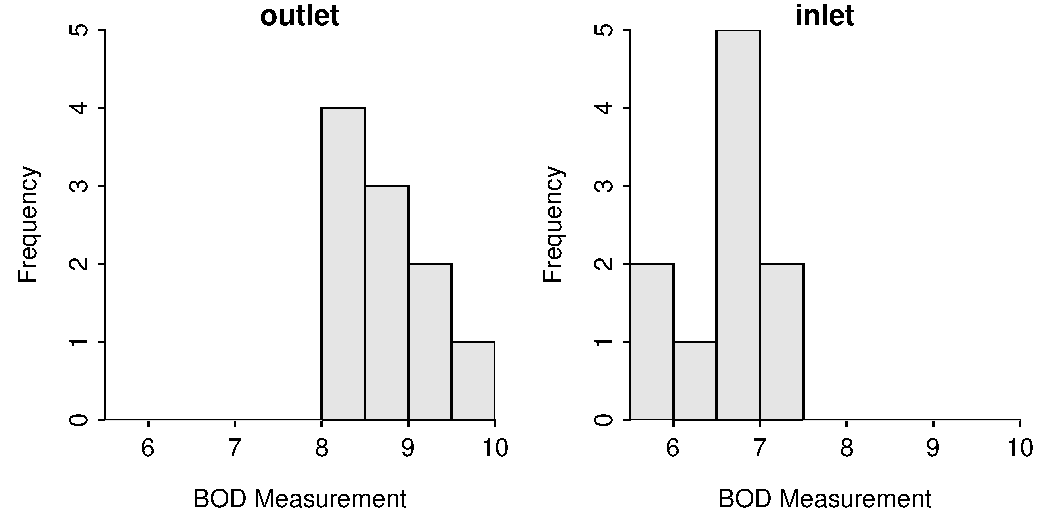
\includegraphics[width=.7\linewidth]{Figs/AquaHist-1} 

}

\caption[Histogram of the BOD measurements at the outlet and inlet of the aquaculture facility]{Histogram of the BOD measurements at the outlet and inlet of the aquaculture facility.}\label{fig:AquaHist}
\end{figure}


\end{knitrout}

\begin{minipage}{\textwidth}
\textbf{R Appendix:}
\begin{knitrout}
\definecolor{shadecolor}{rgb}{0.922, 0.922, 0.922}\color{fgcolor}\begin{kframe}
\begin{verbatim}
aqua <- read.csv("data/BOD.csv")
aqua$src <- factor(aqua$src,levels=c("outlet","inlet"))
hist(BOD~src,data=aqua,xlab="BOD Measurement")
levenesTest(BOD~src,data=aqua)
( aqua.t <- t.test(BOD~src,data=aqua,var.equal=TRUE,alt="greater",conf.level=0.90) )
\end{verbatim}
\end{kframe}
\end{knitrout}
\end{minipage}




%    \cleardoublepage
%    \phantomsection
%    \addcontentsline{toc}{part}{Appendix}
%    \chapter*{Appendices}
%    \appendix


%  \backmatter
%    %BIBLIOGRAPHY ---------------------------------------------------------------------------------------------------------
\cleardoublepage                             %not sure why but this is needed so TOC entry will point to right start page
\phantomsection                              %not sure why but this is needed so TOC entry will point to right start page
\addcontentsline{toc}{part}{Bibliography}    %Add a TOC entry
\bibliography{c:/aaaWork/zGnrlLatex/DHO_Bib} %make the bibliography
 
%INDEX ----------------------------------------------------------------------------------------------------------------
% cross references for the index
\index{Alternative Hypothesis|see{Hypothesis, Alternative}}
\index{Coefficient of Determination|see{$r^{2}$}}
\index{Forward calculation|see{Normal Distribution, Finding areas}}
\index{Frequency Table|see{Table, Frequency}}
\index{Goodness-of-Fit Test|see{Chi-square}}
\index{Line!Finding best-fit|see{Regression}}
\index{Mean!Inference|see{Z-test and t-Test}}
\index{Null Hypothesis|see{Hypothesis, Null}}
\index{Percentage Table|see{Table}}
\index{Proportions Table|see{Table, Proportion}}
\index{Row Proportions Table|see{Table, Proportion}}
\index{Column Proportions Table|see{Table, Proportion}}
\index{Table Proportions Table|see{Table, Proportion}}
\index{Proportions, Inference|see{Chi-square}}
\index{Rejection Criterion|see{$\alpha$}}
\index{Reverse calculation|see{Normal Distribution, Finding values}}
\index{Simple Linear Regression|see{Regression}}
\index{SLR|see{Regression}}
\index{Standard Normal Distribution|see{Normal Distribution}}
\index{Standardization|see{Normal Distribution, Converting to Z-scale}}
\index{One-sample Z-Test|see{Z-Test}}
\index{1-sample Z-Test|see{Z-Test}}
\index{One-sample t-Test|see{t-Test}}
\index{1-sample t-Test|see{t-Test}}
\index{Two-sample t-Test|see{t-Test}}
\index{2-sample t-Test|see{t-Test}}
\index{Matched-Pairs t-Test|see{t-Test}}
\index{Two-way Table|see{Table, Frequency}}
\index{Type I Error|see{Hypothesis Testing, Errors}}
\index{Type II Error|see{Hypothesis Testing, Errors}}
\index{Variability!Natural|see{Natural Variability}}
\index{Variability!Sampling|see{Sampling Variability}}
\index{Variable!Types|see{Quantitative, Continuous, Discrete, Categorical, Nominal, or Ordinal}}
\index{Variance!Testing Equality|see{Levene's Test}}
\index{Y-intercept|see{Intercept}}
\index{Z-Distribution|see{Normal Distribution, Standard Normal}}

% code to actually add the index
\addtocontents{toc}{\setlength{\cftbeforepartskip}{0.4em}}  %decrease dist before parts in back matter portion of TOC
\cleardoublepage                          %not sure why but this is needed so TOC entry will point to right start page
\phantomsection                           %not sure why but this is needed so TOC entry will point to right start page
\addcontentsline{toc}{part}{Index}        %Add a TOC entry
\printindex                               %Make the index


\end{document}
